\section{فعال نمودن قابلیت ها}
در حال حاضر قابلیت نمایش دریفت و اعمال ضریب زلزله در فایل ایتبز در نرم افزار قابل انجام است. هر کدام از آنها را شما میتوانید ۵ مرتبه به صورت رایگان استفاده کنید. نرم افزار بعد از هر بار استفاده تعداد مجاز باقیمانده را به شما یادآوری میکند. بعد از اینکه این سقف تمام شد،
در صورت تمایل به استفاده، میتوانید مطابق پنچره راهنما (مطابق شکل 
\ref{pic:register}
) کدی که نرم افزار به شما میدهد را به همراه فیش واریزی، برای من ارسال کنید. من در اسرع وقت  قابلیت مورد نظر شما را فعال میکنم و به شما اطلاع میدهم. بعد از آن کافیست یکبار در حالی که به اینترنت متصل هستید قابلیت مورد نظرتان را اجرا کنید تا این قابلیت برای شما فعال شود.

در صورتی که تعداد افراد به حد مشخصی برسد، از آن پس این قابلیت برای همگان به صورت رایگان قابل استفاده خواهد بود. پس در صورتیکه نیاز فوری به قابلیت مورد نظرتان ندارید میتوانید تا پرشدن سقف آن صبر کنید تا بتوانید به صورت رایگان از نرم افزار استفاده کنید.

 
 \begin{figure}
     \centering
     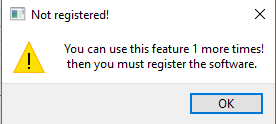
\includegraphics[scale=0.7]{figures/no_of_using}
     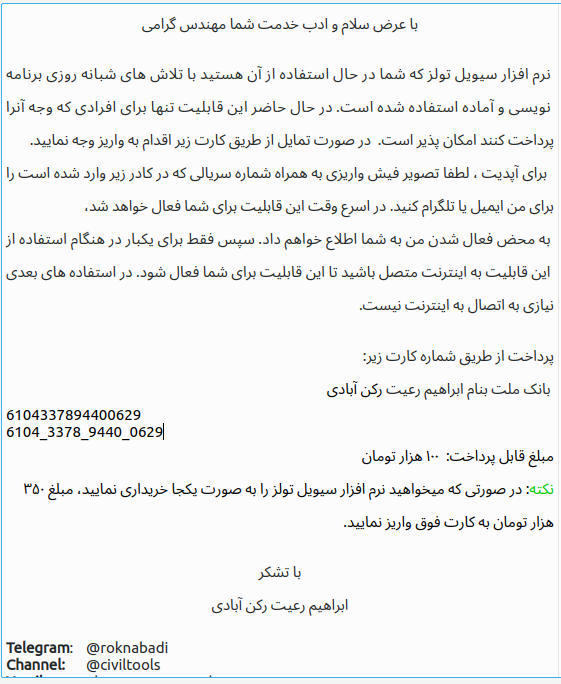
\includegraphics[scale=0.7]{figures/register}
     \caption{توضیح چگونگی فعال کردن قابلیت مورد نظر در نرم افزار}
     \label{pic:register}
 \end{figure}
 
